\documentclass[acmtoms]{acmtrans2m}
\usepackage{graphicx}

% begin definitions and macros

\newcommand{\struct}{{\tt struct}}
\newcommand{\double}{{\tt double}}
\newcommand{\fh}{{\tt function\_handle}}
\newcommand{\mstring}{{\tt string}}

\newcommand{\hs}{\hspace*}
\newcommand{\e}{\hspace*{2 ex}}

\newcommand{\trans}{^{\scriptscriptstyle T}}
\newcommand{\norm}{\|}
\newcommand{\rad}{{\Delta}}
\newcommand{\bord}{B_{\alpha}}
\newcommand{\bormat}{
\left(
\begin{array}{cc}
\alpha & g\trans \\
g & \hessian\\
\end{array}
\right)
}
\newcommand{\onext}{(1,x\trans)\trans}

\newcommand{\philam}{\phi(\lambda)}
\newcommand{\dphilam}{\phi^{\prime}(\lambda)}
\newcommand{\alphaU}{\alpha_{\scriptscriptstyle U}}

\newcommand{\deltao}{\delta_{1}}
\newcommand{\deltaU}{\delta_{\scriptscriptstyle U}}
\newcommand{\noeq}{A\trans{A}}

\newcommand{\trsref}{(\ref{trs})}

\newcommand{\alphaz}{\alpha^{(0)}}
\newcommand{\alphaone}{\alpha^{(1)}}
\newcommand{\alphak}{\alpha^{(k)}}

\newcommand{\tenmt}{10^{\scriptscriptstyle -2}}
\newcommand{\tenmf}{10^{\scriptscriptstyle -4}}
\newcommand{\tenme}{10^{\scriptscriptstyle -8}}
\newcommand{\tenmte}{10^{\scriptscriptstyle -10}}

\newcommand{\matlab}{MATLAB}
\newcommand{\mlstrs}{LSTRS}
\newcommand{\hessian}{H}
\newcommand{\ntn}{n\times n}
\newcommand{\nto}{n\times 1}
\newcommand{\ds}{\displaystyle}

% end definitions and macros

\markboth{Rojas, Santos, and Sorensen \hs{5cm}}{\hs{5cm} LSTRS Software Manual}

\title{Algorithm xxx: LSTRS Software Manual}
\vspace{0.1cm}

\author{MARIELBA ROJAS \\ Technical University of Denmark\\
SANDRA A. SANTOS \\State University of Campinas
\and
DANNY C. SORENSEN \\Rice University
}

\begin{abstract}
The software manual of a\ \matlab\ 6.0 implementation of the LSTRS method is presented.
LSTRS was described in M. Rojas, S.A. Santos and D.C. Sorensen, A new
matrix-free method for the large-scale trust-region subproblem,
{\em SIAM J. Optim.}, 11(3):611-646, 2000. 
LSTRS is designed for large-scale quadratic problems with one norm constraint.
The method is based on a reformulation of the trust-region subproblem as
a parameterized eigenvalue problem, and consists of an iterative
procedure that finds the optimal value for the parameter.
The adjustment of the parameter requires the solution of a large-scale
eigenvalue problem at each step. LSTRS relies on matrix-vector products
only and has low and fixed storage requirements, features that make
it suitable for large-scale computations. In the\ \matlab\ 
implementation, the Hessian matrix of the quadratic objective function
can be specified either explicitly, or in the form of a matrix-vector multiplication
routine. Therefore, the implementation preserves the matrix-free nature of the method.
A description of the\ \matlab\ software, version 1.2, is presented.
A guide for using the software and examples are provided.
\end{abstract}

\category{G.4}{Mathematical Software}{Documentation}
\terms{Algorithms, Design} 
\keywords{ARPACK, constrained quadratic optimization, Lanczos method, regularization, \matlab, trust-region}

            
\begin{document}
\begin{bottomstuff}
Authors's Addresses: 

{\bf M. Rojas}, Informatics and Mathematical Modelling,
Technical University of Denmark, 2800 Kgs. Lyngby,
Denmark ({\tt mr@imm.dtu.dk}). This author was supported in part by
NSF cooperative agreement CCR-9120008, the Research Council of Norway,
and the Science Research Fund of Wake Forest University.

{\bf S.A. Santos}, Department of Applied Mathematics, State
University of Campinas, CP 6065, 13081-970, Campinas, SP, Brazil
({\tt sandra@ime.unicamp.br}). This author was supported by
FAPESP (06/53768-0), CNPq (302412/2004-2), FINEP and FAEP-UNICAMP.

{\bf D.C. Sorensen}, Department of Computational and Applied
Mathematics, Rice University, 6100 Main St., Houston, TX 77005-1892,
USA ({\tt sorensen@caam.rice.edu}).
This author was supported in part by NSF Grants
CCR-0306503, ACI-0325081 and CCF-0634902.
\end{bottomstuff}

\maketitle

% section - Introduction 

\section{Introduction}

This document contains the software manual for version 1.2 of 
a\ \matlab~\cite{matlab} 6.0 implementation
of the LSTRS method~\cite{rss2000} for large-scale
quadratic problems with a quadratic constraint, or trust-region
subproblems:
\begin{eqnarray}
&\min&\ \frac{1}{2} x\trans \hessian x + g\trans x\ {\rm\ subject\ to\ (s.t.)\ }\ \norm x\norm \leq \rad, \label{trs}
\end{eqnarray}
where\ $\hessian$\ is an\ $\ntn$, real, symmetric matrix, $g$\ is
an\ $n$-dimensional real vector,\ $\rad$\ is a positive scalar,
and\ $\norm\cdot\norm$\ denotes the Euclidean norm.

The\ \matlab\ implementation of LSTRS described in this manual allows the
user to specify the matrix
$\hessian$\ both explicitly, a feature that can be useful for small test
problems,
and implicitly, in the form of a matrix-vector multiplication routine, hence
preserving the matrix-free nature of the original method. LSTRS is an iterative
method that requires, at each step, the solution of a parameterized eigenvalue
problem for the {\em bordered} matrix
\[
\bord = \bormat
\]
with $\ds\alpha$\ a scalar parameter. An eigenpair\ $\ds\{\lambda,\onext\}$
of\ $\ds\bord$\ provides points\ $\lambda, \philam = -g\trans x$, and
$\dphilam = x\trans x$, used in rational interpolation schemes
to update the parameter\ $\ds\alpha$.

In the software, several options
are available for the solution of the eigenvalue problems, namely: the 
\matlab\ routine {\tt eig} (QR method), a slightly modified version of
{\tt eigs} (a MEX-file interface for ARPACK \cite{arpack}), a combination
of {\tt eigs} with a Tchebyshev Spectral Transformation,
or a user-provided routine.

The remainder of this document is organized as follows.
In Section~\ref{matlab}, we describe the main features of the software:
data structures, interface, and components. In Section \ref{install}, we provide
instructions for installing and running the software.
In Section~\ref{examples}, we illustrate the use of the software with several examples.

% section - The Matlab Software

\section{The \matlab\ software}\label{matlab}

In this section, we describe our\ \matlab\ 6.0 implementation
of the LSTRS method from \cite{rss2000}. In the following, the
{\tt teletype} font is used for 
\matlab\ codes, built-in types and routines; {\tt\bf boldface}
is used for file names, parameters, variables (including structure fields), and
also to highlight parts of \matlab\ codes.

\subsection{Data structures}\label{datastructures}
The main data structures, implemented with the \matlab\ type \struct,
are the following:
\begin{itemize}
\item A structure for the bordered matrix\ $\bord$,
with fields: {\tt\bf H} (the Hessian matrix), {\tt\bf g} (the gradient vector),
{\tt\bf alpha} (the scalar parameter\ $\alpha$), {\tt\bf dim} (one plus the
dimension of the trust-region subproblem), {\tt\bf bord} (scalar indicating if
the structure represents a bordered matrix (1), or if only the Hessian
is to be used (0)), and {\tt\bf Hpar} (parameters for {\tt\bf H}, whenever
{\tt\bf H} is a matrix-vector multiplication routine, cf. Section \ref{input}).

\item A structure for the LSTRS iterate chosen from two eigenpairs of\ $\bord$.
The fields of the structure are: {\tt\bf lambda} (the eigenvalue), {\tt\bf nu} (the first component of the
eigenvector), {\tt\bf anu} (the absolute value of {\tt\bf nu}), {\tt\bf u}
(an\ $n$-dimensional vector consisting of the last\ $n$\ components of the eigenvector), and
{\tt\bf noru} (the norm of the vector {\tt\bf u}).

\item A structure for the interpolation points, with fields: {\tt\bf lambda} ($\lambda$),\linebreak {\tt\bf fi} ($\philam$),
and {\tt\bf norx} ($\sqrt{\dphilam}$).

\end{itemize}

\subsection{Interface}

The front-end routine is called {\tt\bf lstrs}.
The most general call to this routine is of the form:\\

\noindent\e {\tt
[x,lambda,info,moreinfo] = ...

\noindent\e {\bf lstrs}({\bf H},g,delta,epsilon,{\bf eigensolver},lopts,Hpar,eigensolverpar);\\
}

The parameter {\tt\bf H} specifies either the Hessian matrix
or a matrix-vector multiplication routine; {\tt\bf eigensolver} specifies
the eigensolver routine. The {\em required} input parameters are:
{\tt\bf H, g, delta}. The remaining parameters are {\em optional} with 
default values provided where appropriate. 
A detailed specification of the parameters follows.
The type and default values for the optional parameters are given between
curly brackets.

\subsubsection{Input parameters}\label{input}
\hspace{3cm}

\noindent{\bf Required (3):}
\begin{enumerate}
\item {\tt\bf H} \{\mstring, \fh, or \double\}: matrix-vector multiplication routine,
or an\ $n\times n$\ array containing a symmetric matrix.

\item {\tt\bf g} \{\double\}: $\nto$\ array.

\item {\tt\bf delta} \{\double\}: positive scalar (trust-region radius).
\end{enumerate}

\noindent{\bf Optional (5):}

\begin{enumerate}
\item{\tt\bf epsilon} \{{\tt struct}\}: contains the tolerances for the stopping criteria.
The fields are:
\begin{itemize}
\item {\tt\bf Delta} \{\double, $\tenmf$\}: boundary solutions.
\item {\tt\bf HC} \{\double, $\tenmf$\}: quasi-optimal solutions.
\item {\tt\bf Int} \{\double, $\tenmte$\}: interior solutions.
\item {\tt\bf alpha} \{\double, $\tenme$\}: size of the safeguarding interval for\ $\alpha$.
\item {\tt\bf nu} \{\double, $\tenmt$\}: small components.
\end{itemize}

\item{\tt\bf eigensolver} \{\mstring\ or \fh, {\tt 'eigs\_lstrs\_gateway'}\}: specifies
the eigensolver routine. Current choices for the eigensolver are:
\begin{itemize}
\item User-provided. See Section \ref{eigensolver} for the calling sequence.
\item {\tt\bf eig\_gateway}: gateway to \matlab\ routine {\tt eig}
(QR method).
\item {\tt\bf eigs\_lstrs\_gateway}: gateway to {\tt eigs\_lstrs}, a modified
version of \matlab's {\tt eigs} (ARPACK \cite{arpack} implementation of the Implicitly Restarted Arnoldi Method \cite{sorensen1992}).
The modified routine returns more information, 
including the number of converged eigenvalues and the smallest
Ritz value.
\item{\tt\bf tcheigs\_lstrs\_gateway}: gateway to a routine that computes
the eigenpairs of a given matrix from the eigenpairs of a Tchebyshev matrix polynomial
of degree 10. It is a combination of {\tt\bf eigs\_lstrs} and a
Tchebyshev Spectral Transformation as described in \cite{rs2002}. %The transformation will be
%described in detail in Section \ref{reglstrs}.
\end{itemize}
\item{\tt\bf lopts} \{\struct\}: options for {\tt\bf lstrs} with fields:
\begin{itemize}
\item {\tt\bf maxiter} \{\double, 50\}: scalar indicating the maximum number of LSTRS
iterations allowed.
\item {\tt\bf message\_level} \{\double, 1\}: scalar indicating the level of messages
desired. The options are: no messages (0), a message per iteration
plus a summary at the end (1), and more detailed messages (2).
\item {\tt\bf name} \{\mstring\}: the problem name.
\item {\tt\bf plot} \{\mstring, {\tt 'no'}\}: indicates if a plot of the solution
is desired. The possible values are:
a string beginning with {\tt'{\bf y}'} or {\tt'{\bf Y}'} (plot), or any other
string (no plot).
\item {\tt\bf correction} \{\mstring, {\tt 'yes'}\}: indicates if, in the
hard case, a correction term in the direction of an eigenvector corresponding to the
smallest eigenvalue of the Hessian matrix\ $\hessian$, should be added. 
The possible values are: a string beginning with {\tt'{\bf y}'} or {\tt'{\bf Y}'} (add), or
any other string (do not add).
\item {\tt\bf interior} \{\mstring, {\tt 'yes'}\}: indicates if, when the existence
of an interior solution is detected, such solution should be computed.
The possible values are: 
a string beginning with {\tt'{\bf y}'} or {\tt'{\bf Y}'} (compute), other
string (do not compute).
\item {\tt\bf intsoltol} \{\double, {\tt epsilon.Delta}\}: a scalar indicating
the accuracy with which an interior solution should be computed.
\item {\tt\bf deltaU} \{\mstring\ or \double, {\tt 'rayleigh'}\}: a string indicating how to
initialize\ $\deltaU$ (an upper bound for\ $\deltao$, the smallest eigenvalue of\ $\hessian$), or a scalar with the initial value.
Possible values: {\tt'{\bf rayleigh}'}, a Rayleigh quotient with a random vector;
{\tt'{\bf mindiag}'}, the minimum of the diagonal of\ $\hessian$; or a scalar. 
Note that the {\tt'{\bf mindiag}'} option is only available for problems where the
Hessian is given as an array. For problems where the Hessian is available implicitly as
a matrix-vector multiplication routine, the minimum of the diagonal is still a good choice
to initialize\ $\deltaU$. However, in this case, the user must provide this value.
\item {\tt\bf alpha} \{\mstring\ or \double, {\tt 'min'}\}: a string indicating how to initialize the
parameter\ $\alpha$, or a scalar with the initial value.
Possible values: {\tt'{\bf min}'}, $\alphaz = \min\{0,\alphaU\}$;
{\tt'{\bf deltaU}'}, $\alphaz = \deltaU$; or a scalar.
\item {\tt\bf maxeigentol} \{\double, {\tt [\ ]}\}: the desired maximum relative accuracy
in the eigenpairs, in case the user wants to adjust this accuracy
at each iteration. Possible values are {\tt [\ ]} for no adjustment,
a scalar (maximum relative accuracy),
or a structure containing the maximum relative accuracy of the eigenpairs
({\tt\bf maxeigentol}) and the accuracy of the norm of the current iterate
({\tt\bf itermaxacc}), i.e. $\frac{| \rad - ||x_k|| |}{\rad}$.
Two different adjustment strategies are implemented in the routine
{\tt\bf adjust\_eigentol}.

\item {\tt\bf heuristics} \{\double, {\tt 0}\}: a scalar indicating
if eigenvalues equal to zero and Lanczos vectors (not converged eigenvectors)
should be used to construct an \mlstrs\ iterate. When set to 0, the heuristics
is not used. The strategy is only available in combination with the
eigensolver {\tt\bf 'eigs\_lstrs'}. Possible values: any scalar.
\end{itemize}

\item{\tt\bf Hpar} \{\struct\}: parameters
for {\tt\bf H}, whenever {\tt\bf H} is a matrix-vector multiplication
routine. See Section \ref{mvroutine} for more details.

\item{\tt\bf eigensolverpar} {\{\tt struct}\}: parameters
for the eigensolver routine. 

If the eigensolver is {\tt\bf eigs\_lstrs\_gateway}
or {\tt\bf tcheigs\_lstrs\_gateway},
the parameter {\tt\bf eigensolverpar} should be used as the parameter
{\tt\bf OPTS} in \matlab's {\tt eigs}, which
specifies the options for ARPACK. \mlstrs\ uses the following default values for
{\tt eigs}' options: {\tt\bf eigensolverpar.tol} = $\tenmt$, \linebreak{\tt\bf eigensolverpar.maxit} = 13,
{\tt\bf eigensolverpar.issym~=~1}, and
\linebreak{\tt\bf eigensolverpar.p = 7} (or\ $n+1$\ if\ $n<7$). 
Note that {\tt\bf eigensolverpar.p}
is the number of vectors used by ARPACK, and hence by LSTRS.

The variable {\tt\bf eigensolverpar.v0} allows the user to specify an initial
vector for the Arnoldi/Lanczos process. For \mlstrs, {\tt\bf eigensolverpar.v0}
must be an\ $(~n~+~1~)~\times~1$\ array of type \double. In the software,
the first column of the Lanczos-basis matrix for the bordered
matrix in a given iteration is used as the initial vector
for the Lanczos process on the bordered matrix in the next iteration.
Finally, \mlstrs\ allows a new field {\tt\bf k} to be added to {\tt\bf eigensolverpar}. This
field is used to specify the number of wanted (small) eigenvalues. The default value
for {\tt\bf eigensolverpar.k} is 2. If a number less than 2 is specified, the parameter is set
to 2. A value greater than 2 is allowed.
Note that {\tt\bf eigensolverpar.k} $<$ {\tt\bf eigensolverpar.p} $\leq$\ $n$\ must hold.


\end{enumerate}

All the optional parameters can be set to the empty array {\tt [ ]}. 
This is useful when we want to use the default value for one
parameter but choose the value of the next. In this way,
the value {\tt [\ ]} is used to {\em skip} a parameter.
The order in which the parameters appear in the header of the
function determines which parameter is skipped.
For example, the first {\tt [\ ]} to appear in a calling sequence corresponds
to {\tt\bf epsilon}.


\subsubsection{Calling specifications for the matrix-vector multiplication routine}\label{mvroutine}

If {\tt\bf H} is a matrix-vector multiplication routine, it is called as
{\tt\bf H(v,Hpar)}, where {\tt\bf v} is an\ $\nto$\ array of type \double,
and {\tt\bf Hpar} is a structure containing parameters for
{\tt\bf H}. If\ $\hessian$\ is the Hessian matrix, the routine {\tt\bf H} should compute:\\ 
\centerline{\tt\bf w = $\hessian$ v.}

If {\tt\bf H} does not require any parameters besides {\bf v}, 
\matlab's {\tt\bf varargin} mechanism can be used in the specification
of the function, as in the function {\tt\bf mv} in Figure \ref{mvnopar}.

\subsubsection{Calling specifications for the eigensolver routine}\label{eigensolver}

As explained in Section \ref{input}, the user may provide the eigensolver
routine, which will be called as:
\vspace{0.1cm}

{\tt
\e \e \e [nconv,lambda1,y1,lambda2,y2] = ...

\e \e \e {\tt\bf eigensolver}(Balpha,eigensolverpar);
}
\vspace{0.2cm}

As before, if only {\tt Balpha} is needed as parameter,
\matlab's {\tt\bf varargin} can be used to define the routine, as in:
\vspace{0.1cm}

{\tt
\e \e \e function [nconv,lambda1,y1,lambda2,y2,it,mvp] = ...

\e \e \e {\bf user\_eigensolver}(Balpha,{\tt\bf varargin})
}
\vspace{0.2cm}

The eigensolver routine should return:
\begin{itemize}
\item {\tt\bf nconv}: number of converged eigenvalues.\\[-0.5cm]

\item {\tt\bf lambda1, y1}: the smallest eigenvalue
of\ $\ds\bord$, and a corresponding eigenvector.\\[-0.5cm]

\item {\tt\bf lambda2, y2}: any of the remaining eigenvalues
of\ $\ds\bord$, and a corresponding eigenvector. In practice,
faster convergence can be expected if this eigenvalue is either the second
or a value close to the second smallest eigenvalue.\\[-0.5cm]
\end{itemize}
The eigensolver routine should receive the following input parameters:
\begin{itemize}
\item {\tt\bf Balpha}: a bordered matrix data structure
as described in Section \ref{datastructures}.\\[-0.5cm]

\item {\tt\bf eigensolverpar}: parameters (usually of type \struct)
for the eigensolver routine.
\end{itemize}

\subsubsection{Output parameters}\label{output}
The routine {\tt\bf lstrs} returns four parameters:

\begin{itemize}
\item {\tt\bf x}: the solution to the trust-region subproblem.

\item {\tt\bf lambda}: the corresponding Lagrange multiplier.

\item {\tt\bf info}: an integer representing the result of the computation, with the following possible values:
\begin{itemize}
\item[] 0:  {\tt\bf x} is a boundary solution.
\item[] 1:  {\tt\bf x} is an interior solution.
\item[] 2:  {\tt\bf x} is a quasi-optimal solution.
\item[] -1: an interior solution was detected and, as instructed by the user,
the linear system was not solved, {\tt\bf x} is the current iterate.
\item[] -2:  {\tt\bf x} is an approximation to the solution corresponding to
the last value of\ $\alpha$\ available when the safeguarding interval
could not be further decreased. Note that {\tt\bf x} might contain a correction
term in the direction of an eigenvector corresponding to the smallest eigenvalue of the Hessian matrix.
%, as described in Section \ref{alphaint}. 
Note also that
{\tt\bf x} can take the value empty ({\tt [\ ]}) if there is no iterate available.
\item[] -3: the maximum number of iterations was reached, {\tt\bf x} is the current
iterate, or empty if there is no iterate available.
\item[] -4: it was not possible to compute an iterate. This can happen when
the eigensolver cannot compute the necessary eigenvectors, {\tt\bf x} is empty.
\end{itemize}

\item {\tt\bf moreinfo}: a structure with fields
{\tt\bf exitcond}, {\tt\bf mvp}, {\tt\bf iter}, {\tt\bf solves}, 
{\tt\bf kkt} and {\tt\bf alpha}, which contain, respectively, strings
indicating all the
stopping criteria that were satisfied, the number of matrix-vector products,
the number of LSTRS iterations, the number of calls to the eigensolver,
the value\ $\frac{\norm(\hessian-\lambda I)x + g\norm}{\norm g\norm}$,
and the final value of the parameter\ $\alpha$.
\end{itemize}

\subsection{Global variables}\label{globalvar}
The global variable {\tt\bf mvp\_lstrs} is used to count the number of
matrix-vector products performed. The variable is used only in three routines:
{\tt lstrs\_method} (initialization), {\tt matvec} (update), and
{\tt output}.

\newpage
\subsection{Output}\label{results}

In addition to the output parameters previously described, when the
message level is chosen as 1 or 2, the following information is
displayed: information on each iteration, and at the end,
a summary of cost indicators (iterations, matrix-vector products).
The value\ $\frac{\norm (H -\lambda I)x + g\norm}{\norm g\norm}$\ is 
provided as an indication of
how well the solution pair satisfies this optimality condition.
The Lagrange multiplier\ $\lambda$\ is also displayed.

The program then displays the first stopping criterion that\ $x$\ satisfies.
In case more than one stopping criteria are satisfied, these are
displayed separately.

When {\tt\bf lopts.message\_level} is 1 or 2, the name
(if provided) of the problem, its dimension, and
the value of\ $\rad$\ are displayed at the beginning of the execution, followed
by the name of the eigensolver routine used. Additionally,
a plot of the LSTRS solution (blue on the screen, dashed in
Figure~\ref{phillipsplot}) can be provided, depending on the value
of the input parameter {\tt\bf lopts.plot}. 
This information can be particularly useful
when only {\em one} trust-region problem needs to be solved, as in regularization.
 
\subsection{Files}

The LSTRS software follows a structured, top-down design. The 
\matlab\ M-files containing the components of the software are presented in
Figure \ref{files}.

\begin{figure}[h!tbp]
\begin{tabular}{ll}
{\tt\bf lstrs.m}: &the front-end routine.\\
{\tt\bf lstrs\_method.m}:& the main LSTRS iteration.\\
{\tt\bf init\_up\_bounds.m}: & initializes the upper bounds for\ $\alpha, \deltao$.\\
{\tt\bf b\_epairs.m}: & front-end routine for eigensolver.\\
{\tt\bf adjust\_eigentol.m}: & adjusts the desired relative eigenpair accuracy.\\
{\tt\bf init\_lo\_bounds.m}: & initializes the lower bound for\ $\alpha$.\\
{\tt\bf upd\_deltaU.m}: & updates the upper bound for\ $\deltao$.\\
{\tt\bf adjust\_alpha.m}: & adjusts\ $\alpha$, might need to compute eigenpairs.\\
{\tt\bf convergence.m}: & checks the stopping criteria.\\
{\tt\bf boundary\_sol.m}: & the boundary-solution stopping criterion.\\
{\tt\bf interior\_sol.m}: & the interior-solution stopping criterion.\\
{\tt\bf quasioptimal\_sol.m}: & the quasi-optimal-solution stopping criterion.\\
{\tt\bf upd\_alpha\_safe.m}: & updates the safeguarding interval for\ $\alpha$.\\
{\tt\bf upd\_param0.m}: & updates\ $\alphaz$\ by one-point interpolation scheme.\\
{\tt\bf interpol1.m}: & one-point rational interpolation scheme.\\
{\tt\bf inter\_point.m}: & chooses the interpolation point from two\\
& eigenpairs of the bordered matrix.\\
{\tt\bf safe\_alpha1.m}: & safeguards\ $\alphaone$.\\
{\tt\bf upd\_paramk.m}: & updates\ $\alphak$\ by two-point interpolation scheme.\\
{\tt\bf interpol2.m}: & two-point rational interpolation scheme.\\
{\tt\bf safe\_alphak.m}: & safeguards\ $\alphak$.\\
{\tt\bf output.m}: & sets output parameter and output messages.\\
{\tt\bf cg.m}: & the conjugate gradient method for computing \\
& interior solutions.\\
{\tt\bf correct.m}: &  adds a suitable correction term to the current\\
& iterate in the hard case.\\
{\tt\bf eigs\_lstrs.m}: & a modified version of\ \matlab's {\tt eigs}.\\
{\tt\bf eig\_gateway.m}:& gateway routine for\ \matlab's {\tt eig}.\\
{\tt\bf eigs\_lstrs\_gateway.m}:& gateway routine for {\tt eigs\_lstrs}.\\
{\tt\bf tcheigs\_lstrs\_gateway.m}:& gateway routine for {\tt eigs\_lstrs} combined with a \\
& Tchebyshev spectral transformation.\\
{\tt\bf matvec.m}: & front-end routine for matrix-vector multiplication.\\
{\tt\bf tchmatvec.m}: & front-end routine for multiplication with \\
&  a Tchebyshev matrix polynomial.\\
{\tt\bf quadratic.m}: & evaluates the quadratic objective function in\\
& problem \trsref.\\
{\tt\bf smallnu.m}: & determines if a scalar is small.
\end{tabular}
\caption{LSTRS M-files.}\label{files}
\end{figure}
%\vspace{0.2cm}

The files {\tt\bf mv.m, uutmatvec.m, simple.m, vcalls1.m, icalls.m,}\linebreak
{\tt\bf vcalls2.m} and {\tt\bf regularization.m}, containing the examples
in Section \ref{examples}, are also distributed with the software.
The file {\tt\bf altmatvec.m} contains an alternative matrix-vector multiplication
routine that does not use {\tt\bf varargin}. The file {\tt\bf atamv.m} contains
a matrix-vector multiplication routine for the quadratically-constrained least
squares case, i.e. when the Hessian is the matrix\ $\noeq$,
with\ $A$\ an\ $m\times n$\ matrix and\ $m\geq n$.

\section{Installing and Running the Software}\label{install}

The \mlstrs\ \matlab\ software is distributed as an archive in either tar or zip format in
the files {\tt\bf lstrs.tar} and {\tt\bf lstrs.zip}, respectively. The Unix/Linux command
{\tt tar xvf lstrs.tar} will create a directory {\tt LSTRS} in the current directory 
where all the M-files listed above will be stored. For the zip format we recommend
that the user creates a directory {\tt lstrs-directory} and store the \mlstrs\ files
in that directory.

In either case, the the \mlstrs\ directory should be included in \matlab's search path.
This can be accomplished with one of the following commands:\linebreak
{\tt path(path,'lstrs-directory')} or {\tt addpath 'lstrs-directory'}.


% section - Examples 
\newpage
\section{Examples}\label{examples}

\begin{figure}[h!tbp]
\begin{center}
\fbox{\parbox{4.95in}{
{\tt\small
\%\\
\%   File: mv.m\\
\%   A simple matrix-vector multiplication routine\\
\%   that computes the Identity matrix times a vector {\bf v}\\
\%\\
function $[$w$]$ = {\bf mv}(v,varargin)\\
w = v;\\[-0.4cm]
}
}}
\caption{\small A matrix-vector multiplication routine {\em without}\ additional parameters.}\label{mvnopar}
\end{center}
\end{figure}
\begin{figure}[h!tbp]
\begin{center}
\fbox{\parbox{4.95in}{
{\tt\small
\%\\
\%   File: uutmatvec.m\\
\%   A matrix-vector multiplication routine that\\
\%   multiplies the matrix: (I-2uu') D (I-2uu') times a vector {\bf v}\\
\%   {\bf D} is a diagonal matrix, {\bf u} is a unit vector\\
\%   {\bf uutmatvecpar} is a structure with two fields {\bf d} and {\bf u}\\
\%   containing the vectors that define the matrix\\
\%\\
function $[$w$]$ = {\bf uutmatvec}(v,uutmatvecpar)\\[-0.2cm]

     d = uutmatvecpar.d;\\
     u = uutmatvecpar.u;\\[-0.2cm]

     w = v - 2 * (u'*v) * u;\\
     w = d .* w;\\
     w = w - 2 * (u'*w) * u;\\[-0.4cm]
}
}}
\caption{A matrix-vector multiplication routine {\em with}\ additional parameters.}\label{mvpar}
\end{center}
\end{figure}

\begin{figure}[h!tbp]
\begin{center}
\fbox{\parbox{4.95in}{
{\tt\footnotesize
\%\\
\% File: simple.m\\
\% A simple problem where the Hessian is the Identity matrix.\\
\%

name    = 'Identity';\\
H       = eye(50);\\
g       = ones(50,1);\\
mu      = -3; \e \e \e \e \% chosen arbitrarily\\ 
xexact  = -ones(50,1)/(1-mu);\\
Delta   = norm(xexact); \\[-0.1cm]

\%\\
\% The simplest possible calls to {\bf lstrs}. Default values are used.\\[-0.1cm]
\%\\[-0.1cm]
\% The initial vector for ARPACK is {\bf random}.\\
\% {\bf mv} is the matrix-vector multiplication routine in Figure \ref{mvnopar}.\\
\%\\
$[$x,lambda,info,moreinfo$]$ = lstrs(H,g,Delta);\\
$[$x,lambda,info,moreinfo$]$ = lstrs(@mv,g,Delta);\\

\hspace{4.5cm} $<$ M A T L A B $>$\\
$>>$ simple\\

Problem: no name available.     Dimension: 50.    Delta: 1.767767e+00\\[-0.2cm]

Eigensolver: eigs\_lstrs\_gateway\\[-0.2cm]

LSTRS iteration: 0\\
$||$x$||$: 9.317862e-01, lambda: -6.588723e+00\\
$|||$x$||$-Delta$|/$Delta: 4.729021e-01\\

LSTRS iteration: 1\\
$||$x$||$: 1.767767e+00, lambda: -3.000000e+00\\
$|||$x$||$-Delta$|/$Delta: 2.512148e-16\\

Number of LSTRS Iterations:     2\\
Number of calls to eigensolver: 2\\
Number of MV products:          19\\

($||x||$-Delta)/Delta: 2.512148e-16\\

lambda: -3.000000e+00\\

$||$g + (H-lambda* I)x$||$/$||$g$||$ = 1.159851e-15\\

The vector x is a Boundary Solution\\

Other Stopping Criteria Satisfied:

\hspace{0.5cm} Quasi-optimal Solution
}
}}
\caption{Simple calls to {\tt\bf lstrs}.}\label{simple}
\end{center}
\end{figure}


\begin{figure}[h!tbp]
\begin{center}
\fbox{\parbox{4.95in}{
{\tt\footnotesize
\%\\
\% File: vcalls1.m\\
\% Uses the same data as in Figure \ref{simple}\\
\%\\
\% Eigensolver is {\bf tcheigs\_lstrs\_gateway}, initial vector for ARPACK is {\bf random}\\
\%\\
$[$x,lambda,info,moreinfo$]$ = lstrs(@mv,g,Delta,$[\ ]$,@tcheigs\_lstrs\_gateway);\\
$[$x,lambda,info,moreinfo$]$ = lstrs(@mv,g,Delta,$[\ ]$,'tcheigs\_lstrs\_gateway');\\[-0.1cm]

\%\\
\% Eigensolver is {\bf eig\_gateway}\\
\%\\
$[$x,lambda,info,moreinfo$]$ = lstrs(H,g,Delta,$[\ ]$,@eig\_gateway);\\[-0.1cm]

\%\\
\% Defining {\bf maxiter, message\_level, name}\\
\% Default values are used for the remaining parameters\\
\%\\
lopts.maxiter       = 3;\\
lopts.message\_level = 0;\\
lopts.name          = name;\\[-0.1cm]

$[$x,lambda,info,moreinfo$]$ = lstrs(@mv,g,Delta,$[\ ]$,$[\ ]$,lopts);\\[-0.1cm]

\centerline{***}
\%\\
\% File: icalls.m\\
\% Uses the same data as in Figure \ref{simple}\\
\%\\
\% This call produces an error: {\bf H} must be a matrix, not a routine\\

\hspace{4.5cm} $<$ M A T L A B $>$\\ 

$>>$ $[$x,lambda,info,moreinfo$]$ = lstrs(@mv,g,Delta,@eig\_gateway);\\

??? Error using $==>$ lstrs\\
To use the eigensolver 'eig\_gateway', 'H' must be a matrix !\\
$---------------------------------$\\
\%\\
\% This call produces an error. The string {\bf name} is \\
\% interpreted as the name of an eigensolver routine\\
\%

\noindent\hspace{4.5cm} $<$ M A T L A B $>$\\ 

$>>$ $[$x,lambda,info,moreinfo$]$ = lstrs(@mv,g,Delta,$[\ ]$,name);\\

??? Error using $==>$ lstrs
Undefined eigensolver: 'Identity'. Not in search path.

}
}}
\caption{Valid and invalid calls to {\tt\bf lstrs}.}\label{calls2}
\end{center}
\end{figure}


\begin{figure}[h!tbp]
\begin{center}
\fbox{\parbox{4.95in}{
{\tt\footnotesize
\%\\
\% File: vcalls2.m\\
\% Redefining {\bf struct} parameters.\\
\%\\
\% {\bf uutmatvec} is the matrix-vector multiplication routine in Figure \ref{mvpar}\\
\% {\bf uutmatvecpar} contains the parameters\\
\%

name = '(I-2uu'') D (I-2uu'')';\\
uutmatvecpar.d = rand(50,1);\\
uutmatvecpar.u = rand(50,1);\\
uutmatvecpar.u = uutmatvecpar.u/norm(uutmatvecpar.u);\\
g = rand(50,1);\\
Delta = 1;\\[-0.1cm]

\%\\
\% These statements redefine the values of {\bf epsilon.Delta, epsilon.HC}\\
\% {\bf lstrs} will use the new values\\
\%\\
epsilon.Delta = 1e-3;\\
epsilon.HC    = 1e-8;\\

$[$x,lambda,info,moreinfo$]$ = lstrs(@uutmatvec,g,Delta,epsilon,uutmatvecpar);\\

\%\\
\% These statements redefine the values of {\bf opts.tol, opts.p, opts.v0} for {\bf eigs\_lstrs}\\
\% and {\bf lopts.message\_level, lopts.name}\\
\%\\
epar.tol = 1e-3;\\
epar.p   = 15;\\
epar.v0  = ones(51,1)/sqrt(51);\e \e \e \% Initial vector for ARPACK\\

lopts.message\_level = 2;\\
lopts.name = name;\\

$[$x,lambda,info,moreinfo$]$ = ...\\
lstrs(@uutmatvec,g,Delta,epsilon,$[\ ]$,lopts,uutmatvecpar,epar);\\[-0.1cm]

\%\\
\% The longest possible call to {\bf lstrs}\\
\%\\
$[$x,lambda,info,moreinfo$]$ = ...\\
lstrs(@uutmatvec,g,Delta,epsilon,@tcheigs\_lstrs\_gateway,lopts,uutmatvecpar,epar);\\
}
}}
\caption{Redefining {\tt\bf struct} parameters for {\tt\bf lstrs}.}\label{calls3}
\end{center}
\end{figure}


\begin{figure}[h!tbp]
\begin{center}
\fbox{\parbox{4.95in}{
{\tt\footnotesize
\%\\
\% File: regularization.m\\
\% Computes a regularized solution for problem {\bf phillips} from\\
\% Regularization Tools \cite{hansen1994}, available from http://www.imm.dtu.dk/$\widetilde{\hspace{0.1cm}}$pch\\
\%\\
$[$A,b,xexact$]$ = phillips(300);\\[-0.2cm]

atamvpar   = A;\\
g          = - (b'*A)';\\
Delta      = norm(xexact);\\[-0.2cm]

lopts.name = 'phillips';\\ lopts.plot = 'y';\\
lopts.correction = 'n';\ \ lopts.interior = 'n';\\

epsilon.Delta = 1e-2;

epar.v0 = ones(301,1)/sqrt(301);  \% Initial vector for ARPACK\\[-0.2cm]

\% {\bf atamv} is the routine in Figure \ref{atamv}\\[-0.2cm]

$[$x,lambda,info,moreinfo$]$ = ...\\
lstrs(@atamv,g,Delta,epsilon,@tcheigs\_lstrs\_gateway,lopts,atamvpar,epar);\\[-0.2cm]

\hspace{4.5cm} $<$ M A T L A B $>$\\ 
$>>$ regularization\\[-0.2cm]

Problem: phillips.     Dimension: 300.    Delta: 2.999927e+00\\[-0.2cm]

Eigensolver: tcheigs\_lstrs\_gateway\\[-0.2cm]

LSTRS iteration: 0\\
$||$x$||$: 8.327280e-01, lambda: -6.913002e+01\\
$|||$x$||$-Delta$|/$Delta: 7.224172e-01\\[-0.2cm]

LSTRS iteration: 1\\
$||$x$||$: 1.746167e+00, lambda: -1.768532e+01\\
$|||$x$||$-Delta$|/$Delta: 4.179302e-01\\[-0.2cm]

LSTRS iteration: 2\\
$||$x$||$: 2.935925e+00, lambda: -3.680399e-01\\
$|||$x$||$-Delta$|/$Delta: 2.133441e-02\\[-0.2cm]

LSTRS iteration: 3\\
$||$x$||$: 3.000546e+00, lambda: 1.883676e-03\\
$|||$x$||$-Delta$|/$Delta: 2.064169e-04\\[-0.2cm]

Number of LSTRS Iterations:     \ \ 4\\
Number of calls to eigensolver: \hspace{0.05cm}5\\
Number of MV products:         \ \ \ \ \ \ \ \ 342\\[-0.2cm]

($||$x$||$-Delta)/Delta: 4.441000e-16\\[-0.2cm]

lambda: 1.904289e-03\\[-0.2cm]

$||$g + (H-lambda* I)x$||/||$g$||$ = 2.501468e-05\\[-0.2cm]

The vector x is a Quasi-optimal Solution
}
}}
\caption{Solving a regularization problem with {\tt\bf lstrs}.}\label{regex}
\end{center}
\end{figure}

\begin{figure}[h!t]
\begin{center}
\fbox{\parbox{4.95in}{
{\tt\small
\%\\
\%   File: atamv.m\\
\%   A matrix-vector multiplication routine\\
\%   that computes {\bf A'*A*v}\\
\%\\
function $[$w$]$ = {\bf atamv}(v,A)\\
w = A*v;\\
w = (w'*A)';\\
}
}}
\caption{\small A matrix-vector multiplication routine that computes\ $w=\noeq v$.}\label{atamv}
\end{center}
\end{figure}


\begin{figure}[h!tbp]
\centerline{\includegraphics[scale=0.65]{lstrs-phillips.eps}}
\caption{LSTRS solution plot for regularization problem {\bf phillips}. The
{\bf dashed} curve (LSTRS solution) will appear as {\bf solid blue} on the screen when
LSTRS is executed under \matlab.
The solid curve is the exact solution which has been added to the LSTRS plot
for comparison (the solid curve is {\em not} generated by LSTRS).} \label{phillipsplot}
\end{figure}

\bibliographystyle{acmtrans}
\bibliography{lstrs}

\begin{received}
Received ?; revised ?; accepted ?
\end{received}

\end{document}
